\chapter{CERED}

In this chapter we will describe the process of generating \textbf{C}z\textbf{e}ch \textbf{R}elationship \textbf{E}xtraction \textbf{D}ataset (CERED). We will discuss various decisions that were made during this process and their impacts. 
We will start by characterizing available data and technological resources. \todo{a co dál}



\todo{nějaká návaznost - říct, že popisuju, že budu spojovat wikipedie}


\section{Overview}

The objective is to create a Relationship Extraction dataset for Czech language using distant supervision\todo{link zpátky}. This section is a quick summary for easier orientation in this chapter. Each of these paragraphs is a teaser for one section of this chapter.

First we researched available knowledge bases and Czech corpora to determine which ones will best suit our purpose. We chose Wikimedia projects Wikidata and Czech Wikipedia. 

Next we analysed how we will find mentions of Wikidata relations in Czech Wikipedia. We sketched out first dataflow diagrams and thought about all the different complex aspects of this task.

We continued with choosing technologies that we will use. Aware of the volume and other characteristics of chosen data, we chose Python as the main programming language, spark as a way to speed up the computations and MorphoDita to deal with Czech language. 

\todo{Změnit, když už máme analýzu}
Than we started the implementation and realized that this seemingly simple problem is rather complex. Even though all that we wanted was to get sentences from Wikipedia, find words or phrases, that can have relations, and link those relations from Wikidata, the number of decisions we had to make and obstacles we had to overcome was rather surprising.

\todo{lepší formulace}
As a side project, we implemented a simple viewer, that can present the dataset

\todo{results}



\section{Data sources}

To be able to perform distant supervision, we need to find suitable data - Czech text corpus and a knowledge base. We will explain the requirements and constraints we have on such data and present our options. In this section, we will provide more information on the chosen ones.

The main constraint is quite straightforward, there has to be nontrivial shared set of entities and relations mentioned in text and stored in knowledge base. We expect more fact based texts to be more suitable, leaning towards encyclopedic or journalistic genre \todo{tak špatná věta}. One option is to focus on some subset of Czech National Corpus \footnote{https://www.korpus.cz/}, for example SYN2013PUB, SYN2009PUB and SYN2009PUB are corpora of written journalism. The other option is to lean in the direction of encyclopedic text with Czech Wikipedia.

Our options for knowledge base are limited, to the best of our knowledge, to Wikidata or Google Knowledge graph \footnote{https://developers.google.com/knowledge-graph}. 

We decided to use Czech Wikipedia and Wikidata, mostly because the intersection of information expressed in text data and in structured data seems promissing. \todo{Další důvody.. zmínit že třeba celkem multilinqual? že jde stáhnout? že není blackbox? lepší disambiguita}


\subsection{Czech Wikipedia}

Wikipedia is a multilingual online encyclopedia created and maintained as an open collaboration project by a community of volunteers\cite{wiki:wiki} and we believe anyone reading this article is familiar with Wikipedia. From out point of view Wikipedia is a corpus of text with tagged topics of articles and some entity mentions. Czech Wikipedia contains approximately 440 000 articles and ranks top 30 across all the different language editions of Wikipedia.
\footnote{As of March 2020 according to https://en.wikipedia.org/wiki/List\_of\_Wikipedias}

A dump of Czech Wikipedia is about 1,6GB and 770MB when compressed.

\subsection{Wikidata}

Wikidata is a knowledge base, which acts as central storage of the structured data of Wikipedia and other Wikimedia projects. Just like Wikipedia, this project is freely available and edited by users (and bots). It provides the option to query the database online (for small enough queries), but it is also possible to download the database in standard formats.

The database focuses on \defineterm{items}, which represent objects, entities, concepts, etc.  The first data collected in Wikidata were links to multilingual version of Wikipedia articles on the same topic, the same Wikidata item. Each item was assigned an identifier, prefix Q and unique number, referred to as \defineterm{QID}. A label together with a description of an item should serve as a human readable identifier. Labels, descriptions a optional aliases are language dependant. 

\defineterm{Properties}, another big concept of Wikidata, can be thought of as categories of items (\wikiitem{mother}{P25} implies a category of all mothers) or as relations between items (\wikiitem{Ron Weasley}{Q173998} has a \wikiitem{mother}{P25} \wikiitem{Molly Weasley}{Q3255012}). Each property has its \defineterm{PID}, an identifier consisting of a prefix P and an unique number, and a data type for a value it can be paired with (such as an item, string, url, number or media file). \todo{hezčí formátování wikiitemm}

Information about any item is recorded in statements. Statement is a key-value pair of an property and a value of prescribed data type. For example, for \wikiitem{Ron Weasley}{Q173998} there are seven statements about his siblings:
\begin{itemize}
\item \wikiitem{sibling}{P3373} \wikiitem{Ginny Weasley}{Q187923}, 
\item \wikiitem{sibling}{P3373} \wikiitem{Fred Weasley}{Q13359612},
\item \wikiitem{sibling}{P3373} \wikiitem{George Weasley}{Q13359613} and so on
\end{itemize} . \todo{formating}

Wikidata project contains over 80 000 000 items, which raises requirements on technological resources, that we will need to work efficiently with such data. Json dump of Wikidata takes 110GB of disk space or 37GB if bzip2 compressed.

\section{Analysis}

\begin{figure}[h]\centering
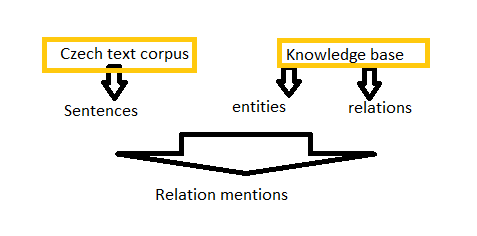
\includegraphics[width=70mm]{./img/Distant}
\caption{Distant supervision diagram}
\label{obr03:Nhust}
\end{figure}

\subsection{Dataflow}

We are starting with two files. One being a Czech Wikipedia dump: it is a collection of articles. Each article has, among other information, its title, id and text. The other is a Wikidata dump. The simpliest way of processing those files would be to process them separately and thus obtaining sentences on one side and relations (a relation type with two items) on the other, see \ref{obr02:AVerySimple}. This approach comes with a clear disadvantage. We would lose any additional information to the sentences, that could be potentially useful (for example article title might be helpful to determine which items are mentioned in a sentence). To solve this we could precompute something for each article and attach it to each sentence, risking a massive increase in required capacity to work with such data. On a similar note, if we were to follow the diagram exactly, we would probably store item names (labels and aliases) in each relation, worsening the situation even further.


\begin{figure}[p]\centering
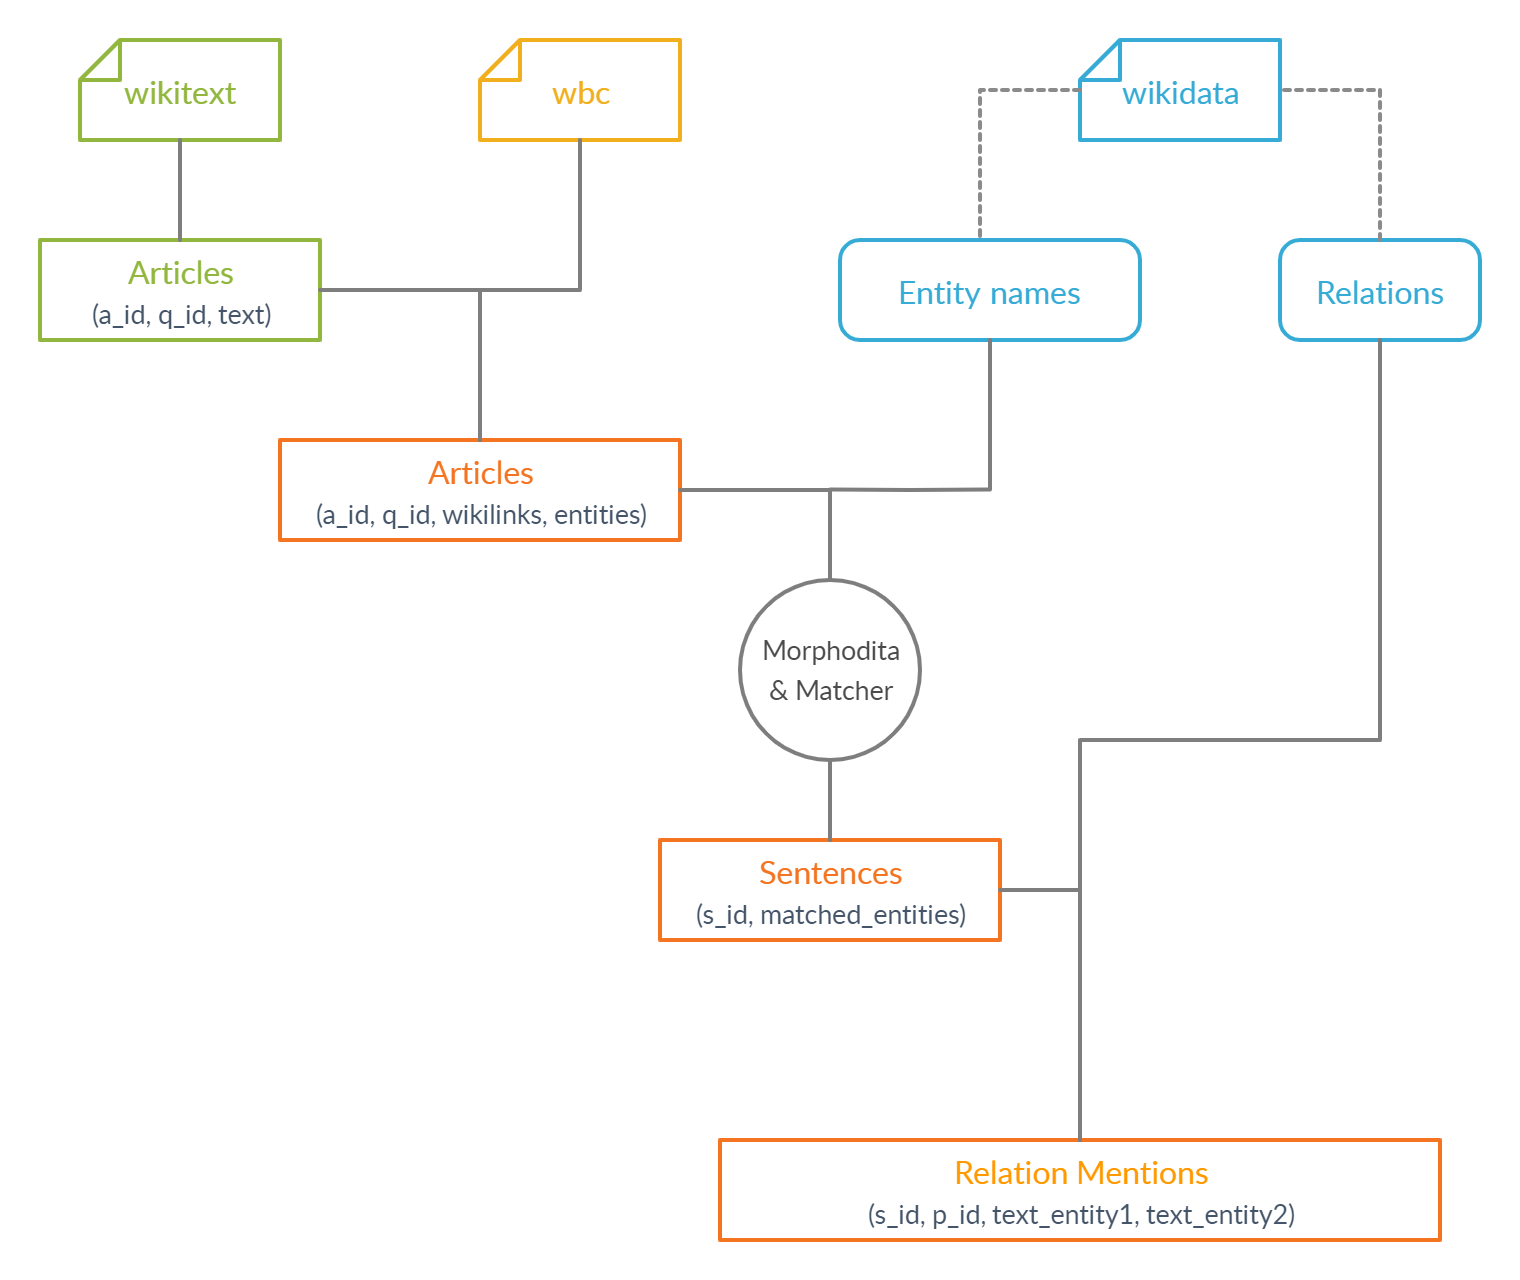
\includegraphics[width=140mm, height=117mm]{./img/Corpus_diagram}
\caption{Zjednodušený diagram výroby korpusu}
\label{obr03:Nhust}
\end{figure}

We decided to update the dataflow to address those issues. We will preprocess Wikidata dump to contain only the data we will use. An item will be kept only if it has a Czech name and we will significantly reduce its statements: we will keep title of its Czech Wikipedia article and create a list of (QID,PID,QID) triples - \defineterm{QPQ}, representing statements that contained information about relations between between this and other items. This way, we have all the necessary information - article title to be able to connect article to item, names for each item to be able to find mentions of items and finally QPQ triples to connect relations and sentences.


Czech Wikipedia maintains a wbc entity usage table, which contains information about which wiki article uses which item. If we use this table, we are able to obtain a list of items, that should be mentioned in an article, lets call this list a \defineterm{wbc candidates}. 






sice by šlo neparalelně, ale co rychlost?

Mluvit o tom, proč nejdřív najdeme, co v článku hledat, pak to nasekáme na věty, pak matchujeme. Zmínit, kolik je jiných možností, že teoreticky by šlo ještě před rozsekáním na věty dělat entity linking ...

Detailně popsat, co kdy kam poteče + diagram

\subsection{WikiManipulace}
Popsat, že wikitext má sám o sobě strukturovaná a divná data a že je to třeba nejspíš řešit

\subsection{Jak teda matchovat entity}

Napsat, že v aj dělají často jen exact modulo zkratky a malé přípony, což tady nejde.

Ukázat nápady se sebráním linků z wikipedie a zavrhnout to

připomenout, jak moc se dá čeština skloňovat
říct, že nemá nejspíš smysl snažit se najít jen validní tvary, protože stejně v textu nejspíš nebudou nevalidní

asi mluvit o word order? a možná i implementovat

Říct, že jako kontrolní dataset budou přímo z linků

\subsection{silver data}
Co to je
proč je nejspíš větší šance na kvalitu
možná i ručně udělat měření kvality na těhle datech v druhé části


\subsection{Distant supervision assumption}
aneb jak matchovat vztahy

\subsection{možná to bude chtít zobrazovátko? aneb jak hodnotit kvalitu?}
možná navrhout nějaké random dotazy na odhalení nevalidních dat?


\subsection{Jaké kategorie?}



\begin{figure}[h]
\begin{center}
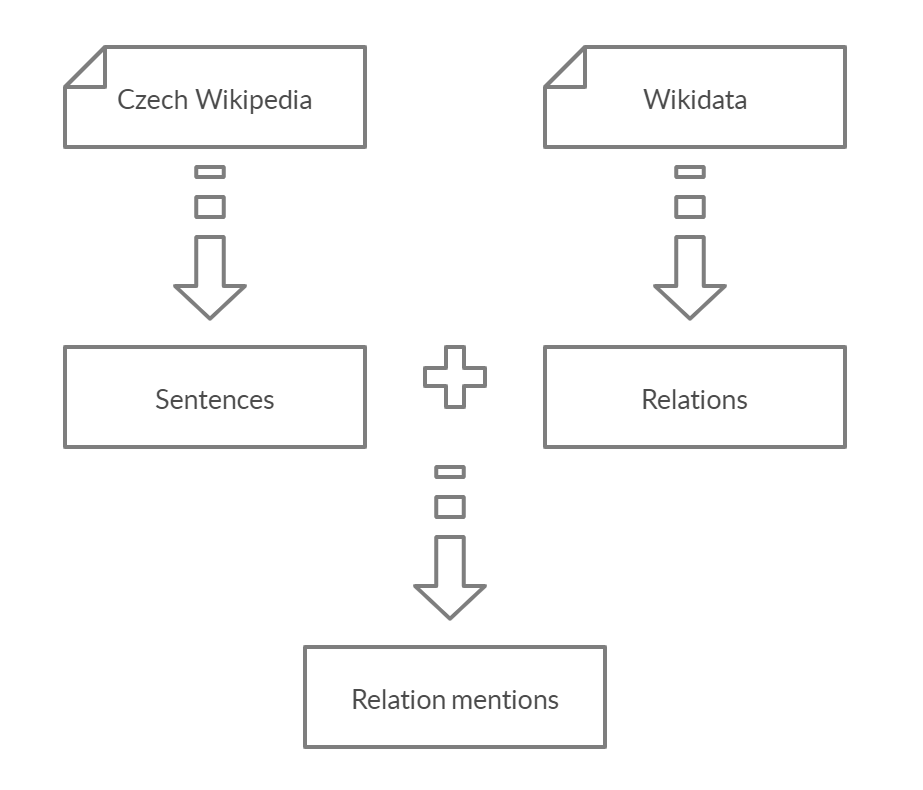
\includegraphics[width=70mm, height=60mm]{./img/a_very_simple_diagram}
\caption{A very simple diagram of dataset generation.}
\label{obr02:AVerySimple}
\end{center}
\end{figure}

\section{Used technologies}
\todo{koukli jsme se na diagram a mysleli, že celé ve spark a tak}
We chose Python to be our main programming language. To be able to work faster with bigger volume of data, we wanted to use a cluster, which leads to Spark and occasionally to some small scripts in shell/bash\todo{co je co?}. To top it, we will use MorphoDita to work with Czech language. Later, we will mention a simple Streamlit app we used to comfortably see results of our Spark queries.

In this section we will briefly introduce those technologies.
\subsection{Python}
\todo{zmiň pandy a numpy a tak}
\subsection{Spark}

\subsection{MorphoDiTa}
MorphoDiTa \cite{Morphodita} (Morphological Dictionary and Tagger) is an open-source tool for morphological analysis of natural language texts. It is designed to work well on inflective languages and achieves state-of-the-art results for Czech language. Internally, during training tries are built to represent patterns for declension. Externally, MorphoDiTa API provides functionalities such as splitting text into sentences, tokenization and lemmatization. 

\subsection{Streamlit}


\section{Implementation}
\section{Viewer}
\section{Results}
